   \subsection{Numerically evaluating $F$}
 
 \label{app:Fnum}
 
 Here I am stealing content from Ref.~\cite{Briceno:2015tza}, where we give some detail between the different expressions for the F-function. First, let us equate the expressions give in Eq.~\ref{eq:Fscdef} and Eq.~\ref{eq:Ffunct_KSS}. To do this, we will explicitly separate the real and imaginary parts of the propagator. The imaginary component is given by the $i \epsilon$ prescription.  We do this using 
\begin{align}
\label{eq:PVdef}
\frac{1}{2 \omega_{a2}(E -  \omega_{a1} - \omega_{a2} + i \epsilon )}
= \frac{\omega_{a1}^*}{E^* (q_a^{*2}-k_a^{*2}+i\epsilon)} + \mathcal S_2
=\frac{\omega_{a1}^*}{E^*}\left[{\rm{P.V.}}\frac{1}{(q_a^{*2}-k_a^{*2})}-i\pi\delta(q_a^{*2}-k_a^{*2})\right] + \mathcal S_2,
\end{align}
where $\mathcal S_2$ is a smooth function that will be annihilated by the sum-integral difference. Here ${\rm{P.V.}}$ denotes the principal-value pole prescription. We further reduce the expression by combining the two spherical harmonics into one
\begin{equation}
4 \pi  Y_{\ell m}(\hat {\textbf k}^*_a)Y^*_{\ell' m'}(\hat {\textbf k}^*_a) =
{4 \pi}\sum_{\ell''m''}
  Y_{\ell'' m''}(\hat {\textbf k}^*_a)
\int d\Omega_{\textbf p}~Y^*_{ \ell m}(\hat {\textbf p}^*_a) Y^*_{\ell'' m''}(\hat {\textbf p}^*_a) Y_{\ell' m'}(\hat {\textbf p}^*_a).
\end{equation}
Putting all the pieces together, we can rewrite Eq.~(\ref{eq:Fscdef}) as Eq.~\ref{eq:Ffunct_KSS}, where $c_{a \ell m}^{{\pmb \Delta}}(q_a^{*2};{L})$ is defined as
\begin{equation}
c_{a \ell m}^{{\pmb \Delta}}(q^{*2}_a;{L})
=
\left[\frac{1}{L^3}\sum_{\mathbf{k}}\hspace{-.5cm}\int~\right]
\frac{\omega_{a1}^*k_a^{*\ell}}{\omega_{a1}}
{\rm{P.V.}}\frac{ \sqrt{4 \pi}  Y_{\ell m}(\hat {\textbf k}^*_a)  }{  k_a^{*2}-q_a^{*2}}.
\end{equation}
Alternatively, this function can be written in terms of the generalized Zeta functions~\cite{Kim:2005gf}
\begin{eqnarray}
\label{eq:clm}
c^{\pmb \Delta}_{a\ell m}(q_a^{*2}; {L})
=\frac{\sqrt{4\pi}}{\gamma L^3}\left(\frac{2\pi}{L}\right)^{\ell-2}\mathcal{Z}^{\pmb \Delta}_{a\ell m}[1;(q_a^* {L}/2\pi)^2],
\hspace{1cm}
\mathcal{Z}^{\pmb \Delta}_{a \ell m}[s;x^2]
= \sum_{\mathbf r \in {\mathcal P}_{{\pmb \Delta}}}\frac{{r}^\ell Y_{\ell m}(\hat {\mathbf{r}})}{(r^2-x^2)^s} \label{eq:clm} \,,
\end{eqnarray} 
where 
\begin{align}
P_{\pmb \Delta} & \equiv  \bigg \{  \, \textbf r \ \bigg \vert \ \textbf r =   \pmb \gamma^{-1}\left( \textbf n - \frac12 \pmb \Delta \right) \,, \ \textbf n \in \mathbb Z^3 \bigg \} \,, \\
\pmb \Delta & \equiv \frac{\textbf P L}{2 \pi} \left (1 + \frac{m_{a1}^2 - m_{a2}^2}{E^{*2}} \right) \,, \\
\pmb \gamma^{-1} \textbf p & \equiv \gamma^{-1} \textbf p_{\parallel} + \textbf p_{\bot} = (E/E^*)^{-1} \textbf p_{\parallel} + \textbf p_{\bot}  \,,
\end{align}
and where $\textbf p_{\parallel}$ and $\textbf p_{\bot}$ are the parallel and perpendicular components of $\textbf p$ with respect to the fixed total momentum $\textbf P$. We close by giving a particularly efficient form for evaluating these quantities~\cite{Leskovec:2012gb},
\begin{multline}
Z_{a\ell m}^{\pmb \Delta}(1,x^2) = \sum_{\textbf r \in P_{\pmb \Delta}} \frac{ r^\ell  Y_{\ell m}(\hat {\textbf r})}{ r^2 - x^2} e^{-( r^2 - x^2)} + \gamma \frac{\pi}{2} \delta_{\ell 0} \delta_{m0} G(x) \\
+ \gamma \pi^{3/2} \int_0^1 dt \frac{e^{tx^2}}{t^{3/2}} \left( \frac{\pi i}{t} \right)^{\ell} \sum_{\textbf n \neq 0} e^{-i \pi \textbf n \cdot \pmb \Delta} \vert \pmb \gamma \textbf n \vert ^{\ell}  Y_{\ell m}( \hat {\pmb \gamma \textbf n}) e^{-(\pi \pmb \gamma \textbf n)^2/t} \,,
\end{multline}
where $\pmb \gamma \textbf p  \equiv \gamma \textbf p_{\parallel} + \textbf p_{\bot}$ and
\begin{equation}
G(x)  \equiv \int_0^1 dt \frac{e^{t x^2} - 1}{t^{3/2}}   - 2  \,.
\end{equation}

where $\alpha=\frac{1}{2}\left[1+\frac{m_1^2-m_2^2}{E^{*2}}\right]$.

{\raul [Task \#3: Write code for $\mathcal{Z}^\mathbf{d}_{lm}$. In other words, drop all of the channel indices. Also, we will only need to think about the case where the masses are degenerate.]}

{\raul [Task \#4: Compare to Eq. 70 in https://arxiv.org/pdf/1202.2145.pdf]}

{\raul [Task \#5: Derive Eq. 70 starting from Eq. 59 in https://arxiv.org/pdf/1202.2145.pdf]}



  %%%%%%%%%%%%%%%%%%%%%%%%%%%%%%%%%%%%%%%%%%
 \subsection{Numerically evaluating $G$}


\label{app:Gnum}

 

\subsubsection{Introduction and general definition \label{sec:Gfunc}}
The goal of this project is to calculate infinite-volume matrix elements of the from
\begin{equation}
\langle \pi \pi ; \mathrm{out}; P_f  \vert \mathcal J_\mu (0) \vert \pi \pi ; \mathrm{in}; P_i \rangle \,,
\end{equation}
where $\mathcal J_\mu$ is a vector current and the states on either side are two-particle asymptotic states with the momentum as indicated. As is described in detail in Ref.~\cite{BH2to2}, one cannot directly measure these matrix elements in a numerical lattice calculation, due to the restriction to finite volume and Euclidean time. It is however possible to extract the matrix elements by combining the following ingredients:
\begin{itemize}
\item The pion vector form factor, $F_{\pi}(Q^2)$, defined via:
\begin{equation}
\langle \pi, p_f \vert \mathcal J_\mu (0) \vert \pi , p_i \rangle = (p_f + p_i)_\mu F_{\pi}(Q^2) \bigg \vert_{Q^2 = (p_f-p_i)^2} \,.
\end{equation}
\item The finite-volume energies with two-pion quantum numbers in various moving frames: $E_n(L, \textbf P)$.
\item The finite-volume matrix elements of states with two-pion quantum numbers in various moving frames:
\begin{equation}
\langle E_{n_f}, \textbf P_f , L \vert \mathcal J_\mu (0) \vert E_{n_i}, \textbf P_i , L \rangle \,.
\end{equation}
\end{itemize}


In order to combine these ingredients and extract the desired quantity, one must calculate a new kinematic function called $G$ and defined by
\begin{multline}
G_{a \ell_f m_{f},a' \ell_f' m_{f}'; b' \ell_i' m_{i}', b \ell_i m_{i}}(P_f,P_i,L)  \equiv \\
\hspace{-4cm}
\delta_{aa'} \delta_{bb'}
\left[\frac{1}{L^3}\sum_{\mathbf{k}}\hspace{-.5cm}\int~\right]
~\frac{1}{2\omega_{a1}}
\frac{ 4 \pi  Y_{\ell_fm_{ f}}(\hat {\textbf k}^*_{af})
Y^*_{\ell_f'm_{f}'}(\hat {\textbf k}^*_{af})
 }{2 \omega_{{a2f}}(E_f -  \omega_{a1} - \omega_{a2f} + i \epsilon )} 
  \bigg (\frac{k^{*}_{af}}{q^*_{af}} \bigg)^{\ell_f+\ell_f'}
\frac{ 4 \pi  Y_{\ell_i' m_{i}'}(\hat {\textbf k}^*_{bi})
Y^*_{\ell_i m_{i}}(\hat {\textbf k}^*_{bi})
 }{2 \omega_{b2i}(E_i -  \omega_{b1} - \omega_{b2i} + i \epsilon )} 
 \bigg (\frac{k^{*}_{bi}}{q^*_{bi}} \bigg)^{\ell_i+\ell_i'}
  \,.
\end{multline}
To evaluate this one takes $E_i, \textbf P_i, E_f, \textbf P_f, L$ and the masses as inputs. For a given point in the summation and integration space, $\textbf k$ should also be viewed as an input. Given these quantities one must first determine $q^{*}_{bi}$, $q^{*}_{af}, k_{bi}^*, k_{af}^*, \hat {\textbf k}^*_{bi}, \hat {\textbf k}^*_{af}$ and the $\omega$s via
\begin{gather}
\sqrt{E_i^2 - \textbf P_i^2} = \sqrt{m_{b1}^2 + q^{*2}_{bi}} + \sqrt{m_{b2}^2 + q^{*2}_{bi}} \,, \hspace{30pt} \sqrt{E_f^2 - \textbf P_f^2} = \sqrt{m_{a1}^2 + q^{*2}_{af}} + \sqrt{m_{a2}^2 + q^{*2}_{af}} \,, \\[5pt]
\begin{pmatrix} \omega_{b1}^* \\ \textbf k_{bi}^*  \end{pmatrix}^{\mu} ={ \Lambda^{\mu}}_{\nu}(- \textbf P_i /E_i) \begin{pmatrix} \omega_{b1} \\ \textbf k   \end{pmatrix}^{\nu} \,, \hspace{30pt} \begin{pmatrix} \omega_{a1}^* \\ \textbf k_{af}^*  \end{pmatrix}^{\mu} ={ \Lambda^{\mu}}_{\nu}(- \textbf P_f /E_f) \begin{pmatrix} \omega_{a1} \\ \textbf k  \end{pmatrix}^{\nu}  \,, \\[5pt]
\omega_{b1} = \sqrt{m_{b1}^2 + \textbf k^2}\,, \ \ \omega_{b2i}  = \sqrt{m_{b2}^2 + (\textbf P_i - \textbf k)^2 } \,, \hspace{30pt} \omega_{a1} = \sqrt{m_{a1}^2 + \textbf k^2}\,, \ \ \omega_{a2f}  = \sqrt{m_{a2}^2 + (\textbf P_f - \textbf k)^2 } \,,
\end{gather}
where ${ \Lambda^{\mu}}_{\nu}(- \textbf P_i /E_i)$ is the boost matrix that takes the four-vector $(E_i, \textbf P_i)$ to its zero-momentum frame. From here one has all building blocks for the integrand and it remains only to sum and integrate.

{\mh [For $M_\pi L =4$, $\textbf P_i = 2 \pi \hat {\textbf z}/L$, $\textbf k = 2 \pi (1,1,0)/L$ calculate $\textbf k^*_i/M_\pi$ as a function of $E_i$.]}

\subsubsection{Reduction for two-pion states}


Here we consider the simplifications that arise for two-pion states. We find it useful to work with the target quantity $[G(L) \cdot w]$, where $w$ is the matrix element of the vector current with single-pion states 
\begin{equation}
w_\mu(P_f - k, P_i - k) \equiv
 \langle \pi; P_f - k \vert \mathcal J_\mu (0) \vert  \pi ; P_i - k \rangle \,, 
\end{equation}
and the $\cdot$ indicates that $w$ is decomposed in spherical harmonics and its indices are contracted with those in $G(L)$. Using Lorentz invariance and current conservation we can rewrite
\begin{equation}
w_\mu(P_f - k, P_i - k) 
  =  (P_f - k + P_i - k)_\mu \  F_\pi (Q^2) \,,
\end{equation}
where $Q^2 = (P_f - P_i)^2$. {\mh [Prove this result.]} Note that the pions are on shell, meaning that $(P_f - k)^2 = (P_i - k)^2 = M_\pi^2$. The scalar quantity $F_\pi$ is called the pion vector form factor.

Next, following the recipe outlined in Ref.~\cite{BH2to2}, we substitute $\textbf k(\textbf k_{f}^*, P_f)$ into $P_f - k$ and we substitute $\textbf k(\textbf k_{i}^*, P_i)$ into $P_i - k$. Here we have dropped the channel indices since we are only considering single-pion states. This substitution defines a new coordinate system for $w_\mu$
\begin{equation}
\label{eq:wstardef}
w^*_\mu(P_f ,\textbf k_{f}^* ; P_i , \textbf k_{i}^*) \equiv \Big [ \big [ P_f - k\big ](\textbf k_{f}^*) + \big [P_i - k \big ](\textbf k_{i}^*) \Big ]_\mu \  F_\pi \big [(P_f - P_i)^2 \big ] \,.
\end{equation}
We are thinking of $ \big [ P_f - k\big ]$ as a function of $\textbf k_{f}^*$, with the exact definition given by 
\begin{equation}
\big [ P_f - k\big ]^\mu(\textbf k_{f}^*) = { \Lambda^{\mu}}_{\nu}(\textbf P_f /E_f) \begin{pmatrix} E^*_f - \omega_{f}^* \\ - \textbf k_{f}^*  \end{pmatrix}^{\nu} \,.
\end{equation}
Since we take these four-vectors to be on shell we know that $\vert \textbf k^*_f \vert = q^*_f$. Starting with $w^*$ as defined in Eq.~(\ref{eq:wstardef}), the procedure outlined in Ref.~\cite{BH2to2} is as follows
\begin{enumerate}
\item We decompose $w^*_\mu(P_f ,\textbf k_{f}^* ; P_i , \textbf k_{i}^*)$ in spherical harmonics via
\begin{equation}
w^*_\mu(P_f ,\textbf k_{f}^* ; P_i , \textbf k_{i}^*) = 4 \pi \, Y^*_{\ell_f' m_f'}(\hat {\textbf k}_{f}^*) \  w^*_{\mu; \ell_f' m_f'; \ell_i' m_i'}(P_f , q_{f}^* ; P_i ,  q_{i}^*) \  Y_{\ell_i' m_i'}(\hat {\textbf k}_{i}^*) \,.
\end{equation}
\item In evaluating $G$ we do not directly use the on-shell value of $w^*_\mu(P_f ,\textbf k_{f}^* ; P_i , \textbf k_{i}^*) $ but instead 
\begin{equation}
\label{eq:wbardef}
\overline w^*_\mu(P_f ,\textbf k_{f}^* ; P_i , \textbf k_{i}^*) \equiv 4 \pi \, Y^*_{\ell_f' m_f'}(\hat {\textbf k}_{f}^*) \bigg ( \frac{k^*_f}{q^*_f} \bigg )^{\ell_f'} \  w^*_{\mu; \ell_f' m_f'; \ell_i' m_i'}(P_f , q_{f}^* ; P_i ,  q_{i}^*) \  Y_{\ell_i' m_i'}(\hat {\textbf k}_{i}^*) \bigg ( \frac{k^*_i}{q^*_i} \bigg )^{\ell_i'} \,.
\end{equation}
\end{enumerate}
{\mh [Suppose $w^* = C ( \hat {\textbf k^*_i}_x^2 + \hat {\textbf k^*_f}_x^2) $, then what is the value of $\overline w^*$?]}

This complicated recipe is required to define an on-shell projection that does not introduce singularities at $\textbf k^*_f = 0$. However, in the present case in turns out that the procedure can be rephrased in a much more straight-forward way. In particular one can show that, for the pion vector form-factor, the corresponding ``barred'' version defined in Eq.~(\ref{eq:wbardef}) reduces to
\begin{equation}
\overline w^*_\mu(P_f ,\textbf k_{f}^* ; P_i , \textbf k_{i}^*) = (P_f - k + P_i - k)_\mu \  F_\pi \big [(P_f - P_i)^2 \big ] \,,
\end{equation}
 with $k^\mu = (\omega_{\textbf k}, \textbf k)^\mu$ defined by the summation and integration coordinate. {\mh [Prove this.]} In other words the steps of re-expressing in terms $\textbf k_{f}^*$ and $\textbf k_{i}^*$, decomposing in harmonics, and inserting factors of $k^*_f/q^*_f$ and $k^*_i/q^*_i$ are all achieved with a simple redefinition of $k^\mu$.

Given this observation, the target quantity, $G(L) \cdot w_\mu$, can be written
\begin{equation}
\label{eq:Gdotw}
[G(L) \cdot w_\mu]_{  \ell_f m_{f},  \ell_i m_{i}}(P_f,P_i,L)  \equiv F_\pi[(P_f - P_i)^2] \left [ (P_f + P_i)_\mu  \ G^S_{ \ell_f m_{f},  \ell_i m_{i}}(P_f,P_i,L)   - 2 G^V_{\mu;  \ell_f m_{f},  \ell_i m_{i}}(P_f,P_i,L)    \right ] \,,
\end{equation}
where
\begin{align}
G_{\ell_f m_{f},  \ell_i m_{i}}^S & \equiv 
 \left[\frac{1}{L^3}\sum_{\mathbf{k}}\hspace{-.5cm}\int~\right]  I_{\ell_f m_{f},  \ell_i m_{i}}(P_f, P_i, \textbf k)
  \,,  \\
  G_{\mu; {\ell_f m_{f},  \ell_i m_{i}} }^V & \equiv 
 \left[\frac{1}{L^3}\sum_{\mathbf{k}}\hspace{-.5cm}\int~\right] k_\mu  I_{\ell_f m_{f},  \ell_i m_{i}}(P_f, P_i, \textbf k)
  \,,  \\
  I_{\ell_f m_{f},  \ell_i m_{i}}(P_f, P_i, \textbf k) & = \frac{1}{2\omega_{\textbf k}}
\frac{ \sqrt{4 \pi}  Y_{\ell_fm_{ f}}(\hat {\textbf k}^*_{f})
 }{2 \omega_{{\textbf P_f - \textbf k}}(E_f -  \omega_{\textbf k} - \omega_{\textbf P_f - \textbf k} + i \epsilon )} 
  \bigg (\frac{k^{*}_{f}}{q^*_{f}} \bigg)^{\ell_f }
\frac{ \sqrt{4 \pi}  
Y^*_{\ell_i m_{i}}(\hat {\textbf k}^*_{i})
 }{2 \omega_{\textbf P_i - \textbf k}(E_i -  \omega_{\textbf k} - \omega_{\textbf P_i - \textbf k} + i \epsilon )} 
 \bigg (\frac{k^{*}_{i}}{q^*_{i}} \bigg)^{\ell_i } \,.
\end{align}
{\mh [Using the definitions above, Prove Eq.~(\ref{eq:Gdotw})]}



\subsubsection{Evaluating $G$ for $P_i^\mu = P_f^\mu$}

{\mh [This section is written for general $G$. Simplify it for the case of pions and a vector current.]}

The approach for evaluating $G$ differs depending on whether or not the two momenta are equal. In this section we describe the approach for the case of $P_i^\mu = P_f^\mu = P^\mu$, equivalently for $Q^2 = 0$. 
We focus here on the integral part of $G$, denoted by $G_I$
\begin{multline}
G_{I; \ell_f m_{f}, \ell_f' m_{f}';  \ell_i' m_{i}',  \ell_i m_{i}}(P)  \equiv \\
\hspace{-4cm}
\int \! \! \frac{d \textbf k}{(2 \pi)^3}
~\frac{1}{8 \omega_{1} \omega_{2}^2} 4 \pi  Y_{\ell_fm_{ f}}(\hat {\textbf k}^* )
Y^*_{\ell_f'm_{f}'}(\hat {\textbf k}^* ) 4 \pi  Y_{\ell_i' m_{i}'}(\hat {\textbf k}^* )
Y^*_{\ell_i m_{i}}(\hat {\textbf k}^* )   \bigg (\frac{k^{*} }{q^* } \bigg)^{\ell_f+\ell_f'+\ell_i+\ell_i'} \left[ \frac{1}{(E -  \omega_{1} - \omega_{2} + i \epsilon )} \right ]^2
  \,.
\end{multline}
We have also already restricted attention to a single channel and dropped the $i$ and $f$ labels since there is only one frame for $P_i^\mu = P_f^\mu = P^\mu$.

We begin by rewriting the integral as 
\begin{equation}
\label{eq:GwithF1}
G_{I}(P)  = 
\int \frac{d \textbf k^*}{(2 \pi)^3} \frac{1}{2 \omega_{1}^*}
\mathcal F(\textbf k^*) (E^* - \omega_1^* + \omega_2^*)^2 \left[  \frac{1}{(E  -  \omega_{1})^2 - \omega_{2}^2 +    i\epsilon}\right ]^2
  \,,
\end{equation}
where we have left the harmonic indices on $G_I$ implicit and where
\begin{equation}
 \mathcal F(\textbf k^*) \equiv  \frac{(E -  \omega_{1} + \omega_{2}  )^2}{4 \omega_{2}^2 (E^* - \omega_1^* + \omega_2^*)^2} 4 \pi  Y_{\ell_fm_{ f}}(\hat {\textbf k}^* )
Y^*_{\ell_f'm_{f}'}(\hat {\textbf k}^* ) 4 \pi  Y_{\ell_i' m_{i}'}(\hat {\textbf k}^* )
Y^*_{\ell_i m_{i}}(\hat {\textbf k}^* )   \bigg (\frac{k^{*} }{q^* } \bigg)^{\ell_f+\ell_f'+\ell_i+\ell_i'}\,.
\end{equation}
Here we have also used the fact that ${d \textbf k}/{\omega_{1}}={d \textbf k^*}/{\omega_{1}^*}$. The next step is to rewrite the double pole in CM frame variables
\begin{equation}
\label{eq:ipolesub}
(E -  \omega_{1})^2 - \omega_{2}^2 = [(E, \textbf P) - (\omega_{1}, \textbf k)]^2 - m_{2}^2 = [(E^*, 0) - (\omega_{1}^*, \textbf k^* )]^2 - m_{2}^2 = (E^* - \omega_{1}^*)^2 - \omega_{2}^{*2} \,.
\end{equation}
Substituting this into Eq.~(\ref{eq:GwithF1}) and also substituting
\begin{equation}
\mathcal F(k^*) \equiv \int \! d \Omega\ \mathcal F(\textbf k^*) \,,
\end{equation}
then gives
\begin{equation}
G_{I}(P)  = 
\int_{0}^\infty \frac{d k^* k^{*2}}{(2 \pi)^3} \frac{1}{2 \omega_{1}^*}
 \frac{\mathcal F( k^*)}{(E^*  -  \omega_{1}^* - \omega_{2}^* +    i\epsilon)^2}
  \,.
\end{equation}

The final step is to observe
\begin{equation}
\frac{1}{E^*  -  \omega_{1}^* - \omega_{2}^* +    i\epsilon} = \frac{H(k^*)}{q^* - k^* + i \epsilon} \,,
\end{equation} 
where $E^{*}=\sqrt{m_1^2+q^{*2}}+\sqrt{m_2^2+q^{*2}}$ and 
\begin{equation}
H(k^*) = \frac{(E^*  +  \omega_{1}^* + \omega_{2}^*)(E^{*2} -  \omega_{1}^{*2} - \omega_{2}^{*2} + 2\omega_{1}^*  \omega_{2}^*)}{ 4 E^{*2}(q^*+k^*)} \,.
\end{equation}
This equality follows from
\begin{align}
(E^{*2} -  \omega_{1}^{*2} - \omega_{2}^{*2} + 2\omega_{1}^*  \omega_{2}^*) (E^{*2} -  \omega_{1}^{*2} - \omega_{2}^{*2} - 2\omega_{1}^*  \omega_{2}^*)
\nn\\
&\hspace{-6cm} =E^{*4}  + (2 k^{*2} + m_1^2 + m_2^2)^2  - 2 E^{*2} (2 k^{*2} + m_1^2 + m_2^2) - 4 ( k^{*2} + m_1^2 ) ( k^{*2} + m_2^2 )  \nn\\
&\hspace{-6cm} =E^{*4} - 2 E^{*2} (m_1^2 + m_2^2) + m^4_1 +m^4_2 -2m^2_1m^2_2-4E^{*2}k^{*2}\nn\\
&\hspace{-6cm} =E^{*2}\left(E^{*2} - 2  (m_1^2 + m_2^2) + \frac{\left(m^2_1 -m^2_2\right)^{2}}{E^{*2}}\right)-4E^{*2}k^{*2}
\nn\\
&\hspace{-6cm} = 4 E^{*2}(q^{*2}-k^{*2}).
\end{align}
Finally, we can rewrite the integral as
\begin{equation}
G_{I}(P)  = 
\int_{-q^*}^\infty d x f(x)
 \frac{1}{(x -    i\epsilon)^2}
  \,,
\end{equation}
where
\begin{equation}
f(x) \equiv   \frac{ (x+q^*)^{2}}{(2 \pi)^3} \frac{1}{2 \sqrt{(x+q^*)^2 + m_1^2}} \mathcal F( x+q^*) H(x+q^*)^2  \,.
\end{equation}


To reduce further we substitute $f(x) = f(x- i \epsilon) - f(0) + f(0) = g(x) (x - i \epsilon) + f(0) $ where $g(x) \equiv [f(x- i \epsilon) - f(0)]/(x - i \epsilon)$ has the same analytic properties as $f(x)$
\begin{equation}
G_I(E) \equiv \int_{-a}^\infty dx  g(x) \frac{1}{(x - i \epsilon)} + f(0) \int_{-a}^\infty dx   \frac{1}{(x - i \epsilon)^2} = \mathcal P \int_{-a}^\infty dx  g(x) \frac{1}{x} + i \pi g(0) - \frac{f(0)}{a} \,.
\end{equation}
Substituting for $g$ we conclude
\begin{equation}
\label{eq:simpresult}
G_I(E) \equiv  \mathcal P \int_{-a}^\infty dx  \frac{f(x) - f(0)}{x^2} + i \pi f'(0) - \frac{f(0)}{a} \,.
\end{equation}


\subsubsection{Evaluating $G$ for $\textbf P_i = \textbf P_f = 0 $} 


The simplest case is given by $E_i \neq E_f$ but $\textbf P_i = \textbf P_f = 0$. Then the quantities defined above reduce to
\begin{align}
G_{\ell_f m_{f},  \ell_i m_{i}}^S & = \bigg [\frac{1}{L^3}\sum_{\mathbf{k}} - \int_{\textbf k} \bigg]
~\frac{1}{(2\omega_{\textbf k})^3} \mathcal P
\frac{ \sqrt{4 \pi}  Y_{\ell_fm_{ f}}(\hat {\textbf k} )
 }{ E_f - 2 \omega_{\textbf k}     } 
  \bigg (\frac{k }{q^*_{f}} \bigg)^{\ell_f }
\mathcal P \frac{ \sqrt{4 \pi}  
Y^*_{\ell_i m_{i}}(\hat {\textbf k} )
 }{ E_i - 2 \omega_{\textbf k}   } 
 \bigg (\frac{k }{q^*_{i}} \bigg)^{\ell_i } +   \delta G^{S, i \epsilon}_{  \ell_f m_{f},  \ell_i m_{i}}(P_f,P_i)      
  \,, \\
  G_{\mu ; \ell_f m_{f},  \ell_i m_{i}}^V & = \bigg [\frac{1}{L^3}\sum_{\mathbf{k}} - \int_{\textbf k} \bigg]
~\frac{k_\mu}{(2\omega_{\textbf k})^3} \mathcal P
\frac{ \sqrt{4 \pi}  Y_{\ell_fm_{ f}}(\hat {\textbf k} )
 }{ E_f - 2 \omega_{\textbf k}     } 
  \bigg (\frac{k }{q^*_{f}} \bigg)^{\ell_f }
\mathcal P \frac{ \sqrt{4 \pi}  
Y^*_{\ell_i m_{i}}(\hat {\textbf k} )
 }{ E_i - 2 \omega_{\textbf k}   } 
 \bigg (\frac{k }{q^*_{i}} \bigg)^{\ell_i } +   \delta G^{V, i \epsilon}_{ \mu ; \ell_f m_{f},  \ell_i m_{i}}(P_f,P_i)      
  \,,
\end{align}
where in the expressions for $G^S$ and $G^V$ here both poles are regulated by a principal-value prescription. The second term, $\delta G^{i \epsilon}$, corrects this to the proper $i \epsilon$-definition of the function.

The separation of pole prescriptions is based on the identity
\begin{equation}
\frac{1}{E - 2 \omega_{\textbf k} + i \epsilon} = \frac{E - 2 \omega_{\textbf k} }{(E - 2 \omega_{\textbf k})^2 +  \epsilon^2} - \frac{i \epsilon}{(E - 2 \omega_{\textbf k})^2 +  \epsilon^2} \,.
\end{equation}
Note that, for very small $\epsilon$, integrating the first term is the same as integrating $\omega_{\textbf k}$ from $m$ up to $E/2 - \delta$ and then from $E/2+\delta$ to $\infty$, with $\delta$ taken arbitrarily small. The second term corresponds to a delta function in the limit of small $\epsilon$. 

In fact we see that, given the assumption $E_i \neq E_f$, the conditions $E_f  = 2 \omega_{\textbf k}$ and $E_f  = 2 \omega_{\textbf k}$ cannot be fulfilled simultaneously. This means that $ \delta G^{S, i \epsilon}_{  \ell_f m_{f},  \ell_i m_{i}}(P_f,P_i,L) $ only depends on the cross terms of one $\delta$-function with one principal value. (The double $\delta$-function term vanishes.) The cross terms can be significantly simplifed
\begin{align}
  \delta G^{S, i \epsilon}_{  \ell_f m_{f},  \ell_i m_{i}}(P_f,P_i)  & = i \pi  \int_{\textbf k} 
~\frac{1}{(2\omega_{\textbf k})^3}  
 \sqrt{4 \pi}  Y_{\ell_fm_{ f}}(\hat {\textbf k} )
    \delta(E_f - 2 \omega_{\textbf k})
  \bigg (\frac{k }{q^*_{f}} \bigg)^{\ell_f }
  \frac{ \sqrt{4 \pi}  
Y^*_{\ell_i m_{i}}(\hat {\textbf k} )
 }{ E_i - 2 \omega_{\textbf k}   } 
 \bigg (\frac{k }{q^*_{i}} \bigg)^{\ell_i }  + (i \leftrightarrow f) \,, \\
 & = \frac{i \pi}{8 \pi^3} \int d \Omega_{\hat {\textbf k}}  \int_0^\infty \frac{dk k^2 }{(2\omega_{\textbf k})^3}  
 \sqrt{4 \pi}  Y_{\ell_fm_{ f}}(\hat {\textbf k} )
    \delta(E_f - 2 \omega_{\textbf k})
  \frac{ \sqrt{4 \pi}  
Y^*_{\ell_i m_{i}}(\hat {\textbf k} )
 }{ E_i - 2 \omega_{\textbf k}   } 
 \bigg (\frac{k }{q^*_{i}} \bigg)^{\ell_i }  + (i \leftrightarrow f) \,, \\
& =  \frac{i }{8 \pi } \delta_{\ell_i \ell_f} \delta_{m_i m_f}     \int_{2M_\pi}^\infty \frac{d(2\omega)   k }{(2\omega)^2}  
    \delta(E_f - 2 \omega )
  \frac{ 1
 }{ E_i - 2 \omega   } 
 \bigg (\frac{k }{q^*_{i}} \bigg)^{\ell_i }  + (i \leftrightarrow f) \,, \\
 & =  \frac{i}{8 \pi}  \delta_{\ell_i \ell_f} \delta_{m_i m_f} \frac{1}{E_i - E_f} \bigg [ \frac{q_f^*}{ E_f^2}  \bigg (\frac{q^*_f }{q^*_{i}} \bigg)^{\ell_i } - \frac{q_i^*}{ E_i^2}  \bigg (\frac{q^*_i }{q^*_{f}} \bigg)^{\ell_i } \bigg ]    \,.
\end{align}
{\mh [Prove this and derive the analogous result for $G^V$.]}

Focusing now on a particular spherical harmonic ($\ell=1, m=0$) we write
\begin{align}
 \mathcal G^S_{zz} (E_f, E_i,L) & \equiv 3 \bigg [\frac{1}{L^3}\sum_{\mathbf{k}} - \int_{\textbf k} \bigg]
~\frac{1}{(2\omega_{\textbf k})^3} \frac{k_z^2}{q^*_f q^*_i} \mathcal P
\frac{1}{ E_f - 2 \omega_{\textbf k}     } 
\mathcal P \frac{ 1 }{ E_i - 2 \omega_{\textbf k}   }  e^{-\alpha^2(E_f - 2 \omega_{\textbf k} ) (E_i - 2 \omega_{\textbf k}  )}  \,, \\
 \delta \mathcal G^{S, i \epsilon}_{zz} (E_f, E_i) & \equiv \frac{i}{8 \pi}   \frac{1}{E_i - E_f} \bigg [ \frac{(q_f^*)^2}{q^*_i E_f^2}  - \frac{(q_i^*)^2}{q^*_f E_i^2}   \bigg ] \,.
\end{align}
Here we have also introduced our approach for evaluating $\mathcal G_{zz}$. Following Ref.~\cite{KSS2005} we introduce exponential damping factors with some constant $\alpha$ that has units of length. This damping is expected to introduce artifacts that scale as $e^{- L/\alpha}$ and vanish for $\alpha \to 0$. The function $ \mathcal G^S_{zz} (E_f, E_i,L)$ is plotted in Figure \ref{fig:Gplot} for $\alpha = 0.5$ and $M_\pi L=6$.
{\mh [Write code to check my code for $G^S$ and also to calculate $G^V]$}
 


\begin{figure}
\begin{center}
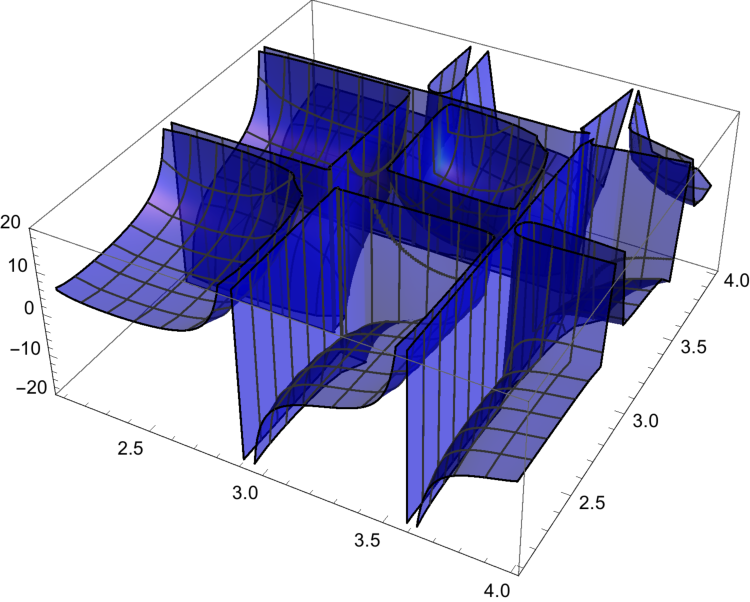
\includegraphics[width=0.4\textwidth]{figs/G3D} \hspace{30pt}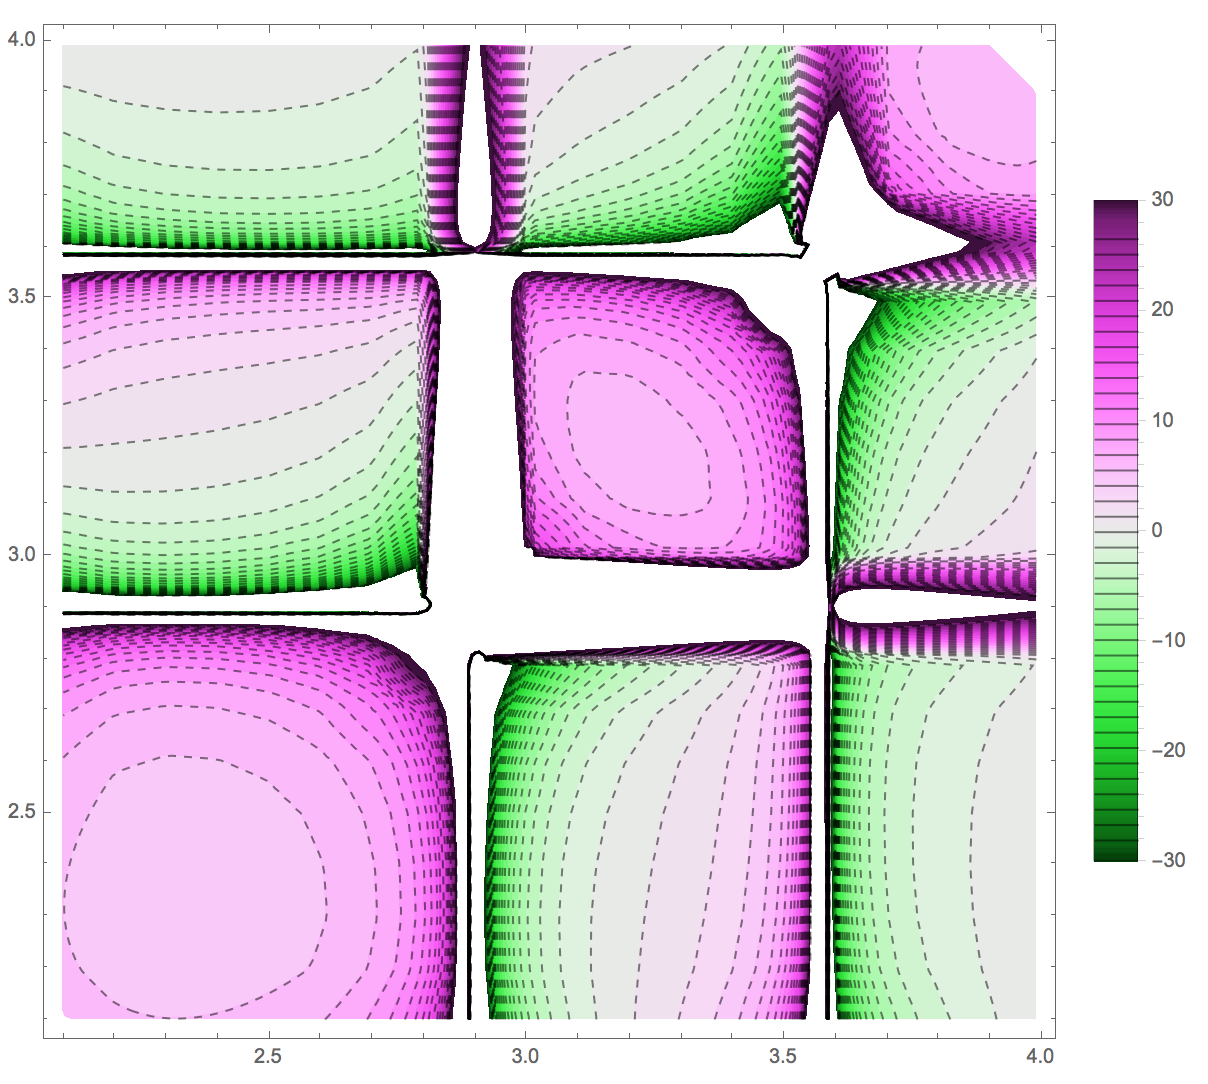
\includegraphics[width=0.35\textwidth]{figs/Gcontour}
\caption{$\mathcal G_{zz}(E_i,E_f,L)$ plotted as a function of $E_i, E_f$ in units of $M_\pi$, with $L$ fixed at $M_\pi L=6$. The singularities arise when either $E_i$ or $E_f$ (or both) coincide with one of the non-interacting two-pion energies. For interacting pions one must sample this function at the finite-volume energies (away from the poles) to determine $\mathcal G_{zz}$. Multiplying this with the pion vector form factor then gives the term needed to extract the $\textbf 2 + \mathcal J \to \textbf 2$ matrix element.
%
\label{fig:Gplot}}
\end{center}
\end{figure}
